\documentclass[11pt,a4paper]{article}
\usepackage[utf8]{inputenc}
\usepackage[T1]{fontenc}
\usepackage{times}
\usepackage{graphicx}
\usepackage{amsmath,amssymb}
\usepackage{booktabs}
\usepackage{multirow}
\usepackage{xcolor}
\usepackage{hyperref}
\usepackage{caption}
\usepackage{subcaption}
\usepackage{tikz}
\usepackage{pgfplots}
\pgfplotsset{compat=1.18}
\usepackage[margin=2.5cm]{geometry}
\usepackage{enumitem}
\usepackage{natbib}
\bibliographystyle{plainnat}

\newcommand{\edd}{\textsc{EDD}}
\newcommand{\atlas}{\textsc{Atlas}}

\title{Ordinal Depth Estimation for Recursive Language Model Generations:\\A Depth Degradation Atlas Across Scales and Strategies}

\author{Anonymous}
\date{}

\begin{document}
\maketitle

% ============================================================
% ABSTRACT
% ============================================================
\begin{abstract}
Web-scraped training corpora increasingly contain text produced by repeated model-to-data-to-model feedback loops, yet existing detectors only answer whether text is machine-generated, not how many recursive cycles it has undergone. We formalize \emph{ordinal generation depth estimation} as a new task: given a passage, predict its recursive generation depth $d \in \{0,1,2,3\}$. We construct a multi-generational benchmark spanning three model families (1B--14B parameters), three decoding strategies, and four depths, then build the first \emph{Depth Degradation Atlas}, a systematic empirical map of how text statistical properties evolve across recursive depths, models, and strategies. Random Forest classifiers on 19 statistical features extracted from a fixed reference model achieve 70--85\% four-class accuracy (chance = 25\%). The Atlas reveals that perplexity tail statistics (\texttt{p90\_ppl}, \texttt{var\_surprisal}) are universal depth markers across all settings, that inter-depth discriminability decays monotonically (formalized as the Effective Discriminable Depth, \edd), and that temperature sampling induces a feature trajectory reversal that breaks naive cross-strategy transfer. We address this reversal with a two-stage pipeline (strategy identification followed by strategy-conditioned depth classification) that achieves 75.2\% mean accuracy, outperforming naive pooling by 3.2 percentage points. The depth signal persists under topic-seeded prompted generation (92.8\% accuracy retention) and at the 14B scale without quantization, confirming ecological relevance and scale robustness.
\end{abstract}

% ============================================================
% 1  INTRODUCTION
% ============================================================
\section{Introduction}

Large Language Models (LLMs) are now prolific generators of web content. When this content is scraped and fed back into training corpora, it creates recursive feedback loops in which models train on their own outputs, or outputs of earlier model generations. Recent theoretical and empirical work has shown that such loops drive \emph{model collapse}: progressive loss of distributional diversity, tail truncation, and convergence toward low-entropy attractors~\citep{shumailov2024ai,alemohammad2024selfconsuming,dohmatob2024tale,gerstgrasser2024model}. The practical consequence is clear. Training data quality degrades as recursive synthetic content accumulates, and curators need tools to detect and manage this contamination.

Existing approaches to machine-generated text detection frame the problem as a binary classification task: is a given passage human-written or machine-generated~\citep{mitchell2023detectgpt,hans2024binoculars,bao2024fastdetectgpt}? While useful, binary labels discard critical information. First-generation synthetic data may be high quality and even beneficial for training~\citep{gunasekar2023textbooks}, whereas deeply recursive text is demonstrably degraded. A curator who can distinguish depth-1 from depth-3 text can make graduated decisions (retain, downweight, or discard) rather than applying a single threshold.

No prior method estimates ordinal generation depth from text alone. Model collapse studies characterize degradation patterns but assume depth is known a priori~\citep{drayson2025investigating,shumailov2024ai}. EditLens~\citep{liang2024monitoring} estimates single-pass AI editing extent but does not address recursive depth. Watermarking schemes~\citep{kirchenbauer2023watermark} require generator cooperation and do not survive retraining cycles. There is a methodological gap between knowing that recursive collapse happens and being able to measure how deep a given text sits in the feedback chain.

We address this gap with three contributions. First, we formalize ordinal generation depth estimation as a classification task and construct a controlled multi-generational benchmark spanning three model families (Pythia-1.4B, OLMo-1B, GPT-2 XL), three decoding strategies (nucleus, temperature, top-k), and four recursive depths ($d \in \{0,1,2,3\}$). We show that Random Forest classifiers on 19 statistical features from a fixed reference model achieve 70--85\% four-class accuracy across all nine model-strategy configurations. Second, we provide the first \emph{Depth Degradation Atlas}: a systematic empirical characterization of how statistical properties evolve across depths, models, and strategies. The Atlas reveals universal depth markers (perplexity tail statistics consistently rank among the top four features), monotonically decaying inter-depth discriminability (formalized as the Effective Discriminable Depth, \edd), and a strategy-dependent feature trajectory reversal caused by temperature sampling's accelerated convergence to the attractor distribution. We extend this Atlas to the 14B scale (Qwen2.5-14B, clean FP16 without quantization confounds) and to prompted generation (topic-seeded text), confirming that the depth signal is neither scale-limited nor an artifact of unconditional generation. Third, we propose a two-stage pipeline for cross-strategy deployment: a strategy identification classifier (81.2\% accuracy on 28 features) routes samples to strategy-conditioned depth classifiers, achieving 75.2\% mean accuracy and outperforming naive pooling by 3.2 percentage points.

% ============================================================
% 2  RELATED WORK
% ============================================================
\section{Related Work}

\paragraph{Model Collapse and Recursive Generation.}
\citet{shumailov2024ai} demonstrated that iteratively retraining language models on their own outputs leads to progressive distributional collapse and loss of tail diversity. Subsequent work formalized convergence rates~\citep{dohmatob2024tale,gerstgrasser2024model} and showed that even partial synthetic contamination accelerates collapse~\citep{alemohammad2024selfconsuming}. \citet{drayson2025investigating} provided empirical characterizations of degradation trajectories across model families. These studies assume generation depth is known, as they control the recursive pipeline. Our work complements this line by estimating depth from text when the generation history is unavailable.

\paragraph{Machine-Generated Text Detection.}
Binary detectors distinguish human-written from machine-generated text using statistical divergence (DetectGPT~\citep{mitchell2023detectgpt}, Fast-DetectGPT~\citep{bao2024fastdetectgpt}), likelihood ratios (Binoculars~\citep{hans2024binoculars}), or learned classifiers (LOKI~\citep{li2024loki}). DivEye~\citep{liang2024diveye} detects synthetic text via n-gram diversity features. These methods produce a single binary or continuous score and do not capture the ordinal structure of recursive generation. Our feature extraction pipeline builds on similar statistical signals (perplexity, surprisal) but targets a multi-class ordinal prediction.

\paragraph{Decoding Strategy Effects.}
\citet{holtzman2020curious} showed that decoding strategy fundamentally shapes the statistical properties of generated text, with nucleus sampling producing more human-like distributions than pure top-k or temperature scaling. \citet{garcesarias2025decoding} recently confirmed that strategy effects interact with model architecture in detection tasks. Our Atlas extends this finding to the recursive setting, revealing that temperature sampling accelerates convergence to the attractor distribution, causing feature trajectory reversal relative to nucleus and top-k strategies.

\paragraph{Authorship and Source Attribution.}
Multi-class attribution of text to specific models or human authors has been studied in stylometry~\citep{uchendu2020authorship} and multi-source detection~\citep{li2024mage}. These methods identify \emph{which} model generated a text, not \emph{how many recursive cycles} it has undergone.

\paragraph{Data Curation and Quality Scoring.}
Data selection methods like DSIR~\citep{xie2023data} and QuRating~\citep{wettig2024qurating} score training examples by distributional proximity to a target or by quality dimensions. Our depth estimates provide a complementary signal: a graduated quality proxy that captures recursive contamination rather than topical fit.

\paragraph{Watermarking.}
Statistical watermarks~\citep{kirchenbauer2023watermark} embed detectable signals into generated text. While effective for single-generation attribution, watermarks do not survive the retraining step in recursive feedback loops and require generator cooperation.

% ============================================================
% 3  TASK FORMALIZATION AND METHOD
% ============================================================
\section{Task Formalization and Method}

\subsection{Problem Definition}

Let $M_0$ be a pretrained language model and $\mathcal{D}_0$ a corpus of human-written text. Define the recursive generation chain:
\begin{align}
    \mathcal{D}_{d+1} &= \text{Generate}(M_d, S), \quad M_{d+1} = \text{FineTune}(M_0, \mathcal{D}_{d+1})
\end{align}
where $S$ is a decoding strategy (nucleus, temperature, or top-k) and $d \in \{0, 1, 2, \ldots\}$ is the generation depth. Depth 0 denotes human-written text. Given a text passage $x$ with unknown depth $d^*$, the task is to predict $\hat{d} = f(x)$ where $f$ maps text to an ordinal depth class.

\subsection{Benchmark Construction}

We construct recursive generation chains for three model families: Pythia-1.4B~\citep{biderman2023pythia}, OLMo-1B~\citep{groeneveld2024olmo}, and GPT-2 XL~\citep{radford2019language}. Each model is fine-tuned using LoRA~\citep{hu2022lora} on its own generated text, then generates the next depth's corpus. We apply three decoding strategies: nucleus sampling ($p=0.95$), temperature sampling ($\tau=0.9$), and top-k sampling ($k=50$). This yields a $3 \times 3$ grid of 9 model-strategy configurations, each producing depths $d \in \{0, 1, 2, 3\}$. We additionally extend the chain to $d \in \{0, \ldots, 5\}$ for depth limit analysis.

For scale validation, we construct a separate chain using Qwen2.5-14B~\citep{yang2024qwen2} in clean FP16 (no quantization) with LoRA fine-tuning and nucleus sampling. For ecological validity, we generate topic-seeded text using GPT-2 XL conditioned on 50 diverse topic prompts spanning science, politics, creative writing, business, and health domains.

\subsection{Feature Extraction}
\label{sec:features}

For each passage $x$, we compute token-level log-probabilities under a fixed reference model (Pythia-1.4B) and extract 19 statistical features organized into four families:

\begin{itemize}[nosep,leftmargin=1.5em]
    \item \textbf{Perplexity distribution} (7 features): mean, standard deviation, median, p75, p90, interquartile range, and max of per-token perplexity.
    \item \textbf{Surprisal statistics} (5 features): mean, variance, skewness, kurtosis, and range of per-token surprisal ($-\log p(x_t | x_{<t})$).
    \item \textbf{Diversity metrics} (4 features): type-token ratio, hapax legomena ratio, bigram entropy, and trigram entropy.
    \item \textbf{Fluency indicators} (3 features): mean log-probability, fraction of tokens with $p < 0.01$, and consecutive low-probability token count.
\end{itemize}

The reference model is held fixed across all experiments to ensure that feature values reflect properties of the text rather than the generating model. When evaluating text generated by Pythia-1.4B itself, we note that cross-scale analysis (Section~\ref{sec:scale}) demonstrates that Pythia-1.4B retains discriminative power even on 14B-generated text, with accuracy within 2--4 percentage points of the within-scale setting.

For the two-stage pipeline (Section~\ref{sec:twostage}), we augment these 19 features with 9 additional strategy-discriminative features: vocabulary coverage ratio, token probability entropy, mean top-1 probability, bigram repetition ratio, hapax legomena ratio (on probability-weighted tokens), top-10 probability mass, Zipf's alpha, unique bigram ratio, and mean token rank.

\subsection{Classification}

We train Random Forest (RF) classifiers with 500 trees and Logistic Regression (LR) baselines using 5-fold stratified cross-validation. For ordinal structure, we additionally evaluate pairwise binary classifiers at each adjacent depth boundary ($d$ vs $d{+}1$), reporting Area Under the ROC Curve (AUC) as the primary discrimination metric.

\subsection{Effective Discriminable Depth (\edd)}
\label{sec:edd}

We define the Effective Discriminable Depth as the maximum depth $d^*$ such that all adjacent-depth binary classifiers up to $d^*$ exceed an AUC threshold $T$:
\begin{align}
    \edd(T) &= \max \{ d^* : \text{AUC}(d \text{ vs } d{+}1) \geq T, \; \forall \, d < d^* \}
\end{align}
We report \edd{} at thresholds $T \in \{0.65, 0.70, 0.75, 0.80\}$ to characterize sensitivity. At $T = 0.75$, seven of nine model-strategy configurations achieve $\edd \geq 3$, indicating that at least three adjacent-depth boundaries are reliably discriminable.

% ============================================================
% 4  THE DEPTH DEGRADATION ATLAS
% ============================================================
\section{The Depth Degradation Atlas}
\label{sec:atlas}

The Depth Degradation Atlas is a systematic empirical map of how text statistical properties evolve across recursive depths. We organize findings along three axes: feature universality, inter-depth discriminability, and strategy-dependent interaction effects.

\subsection{Feature Universality}

Across all nine model-strategy configurations in the 1B benchmark, \texttt{p90\_ppl} (90th percentile of per-token perplexity) and \texttt{var\_surprisal} (variance of per-token surprisal) consistently rank among the top four features by Random Forest importance. This pattern extends to the 14B scale (Table~\ref{tab:scale}), where these two features retain their top-2 ranking (importances 0.185 and 0.162, respectively), and to prompted generation (Table~\ref{tab:prompted}), where they again occupy positions 1 and 2 (importances 0.195 and 0.188). The consistency of tail perplexity statistics as depth markers across model families, parameter counts, and generation modes constitutes a core finding of this work.

\subsection{Monotonic Discriminability Decay}

Adjacent-depth discrimination decays monotonically with depth. In the 1B benchmark, $d_0$ vs $d_1$ AUC ranges from 0.981 to 0.998 across all configurations; $d_1$ vs $d_2$ AUC ranges from 0.713 to 0.937; $d_2$ vs $d_3$ AUC ranges from 0.623 to 0.883. The 14B experiment confirms this pattern: $d_0$v$d_1$ AUC = 0.991, $d_1$v$d_2$ AUC = 0.867, $d_2$v$d_3$ AUC = 0.793 (Table~\ref{tab:scale}). This decay reflects the progressive convergence of the generated distribution toward a low-entropy attractor: each recursive fine-tuning step compresses the distribution, and the marginal compression diminishes as the distribution approaches the attractor.

For depth extension analysis, $d_3$ vs $d_4$ AUC clusters near 0.75 across the three 1B models (Pythia: 0.784, $p=0.001$; OLMo: 0.765, $p=0.091$; GPT-2 XL: 0.750, $p=0.505$), while $d_4$ vs $d_5$ AUC uniformly falls below 0.70 (0.681--0.694). We report these with full confidence intervals and $p$-values rather than claiming uniform statistical significance.

\subsection{Strategy-Dependent Feature Trajectory Reversal}
\label{sec:reversal}

The Atlas reveals a qualitative interaction between decoding strategy and depth. Under nucleus ($p=0.95$) and top-k ($k=50$) sampling, features evolve monotonically with depth: perplexity tail statistics decrease, diversity metrics contract, and surprisal variance narrows. Temperature sampling ($\tau=0.9$) preserves the direction at the $d_0$/$d_1$ boundary but reverses the $d_1$/$d_2$ feature trajectory relative to the other strategies. This reversal is visible in cross-strategy leave-one-out (LOO) experiments: when a classifier trained on nucleus and top-k data is evaluated on temperature-sampled text, the $d_1$ vs $d_2$ AUC drops to 0.13 (GPT-2 XL) and 0.25 (OLMo), indicating that the decision boundary is oriented in the wrong direction.

The root cause is a genuine structural distributional shift. Temperature scaling uniformly divides logits by $\tau$, flattening the probability distribution across the entire vocabulary. In contrast, nucleus and top-k truncate the distribution, preserving the shape of the included portion. Uniform flattening accelerates convergence to the attractor distribution: temperature depth-$N$ features approximate nucleus/top-k depth-$(N{+}1)$ features. For GPT-2 XL, the median \texttt{p90\_ppl} at temperature depth 1 (92.2) falls squarely within the nucleus/top-k depth-2 range (65--92).

This shift cannot be resolved by simple feature normalization. Z-score standardization improves overall LR cross-strategy accuracy from 25\% to 61\%, but does not recover pairwise $d_1$v$d_2$ AUC (GPT-2 XL: 0.50 $\to$ 0.24; OLMo: 0.50 $\to$ 0.19). The worsening AUC under normalization confirms a geometric rotation of the feature space, not a rescalable offset. Whether more sophisticated domain adaptation methods could recover this boundary remains an open question.

We categorize the three strategies into distinct tiers: nucleus serves as a stable baseline with consistent feature trajectories; temperature enhances signal magnitude at shallow depths but induces the $d_1$/$d_2$ reversal in cross-strategy settings; top-k attenuates signal strength but preserves directional consistency.

% ============================================================
% 5  EXPERIMENTS
% ============================================================
\section{Experiments}

\subsection{1B Benchmark: 3-Model $\times$ 3-Strategy Grid}

Table~\ref{tab:benchmark} summarizes four-class RF accuracy across the nine configurations in the 1B benchmark. Accuracy ranges from 69.6\% (OLMo, top-k) to 85.4\% (GPT-2 XL, temperature), with all configurations substantially above the 25\% chance level. GPT-2 XL achieves the highest accuracy across all three strategies, likely due to its larger effective capacity among the 1B-class models.

Per-class recall shows a consistent pattern: $d_0$ recall exceeds 97\% in all settings (the human-vs-machine boundary is easy), while $d_2$ recall is the lowest (26.8--63.0\%), reflecting the compressed inter-depth distances at middle depths. Three-class accuracy excluding $d_0$ ranges from 59\% to 82\%, providing a conservative estimate of ordinal depth estimation performance isolated from the binary detection component.

\begin{table}[t]
\centering
\caption{Four-class Random Forest accuracy (\%) on the 1B benchmark. All values from 5-fold stratified cross-validation. Chance level = 25\%.}
\label{tab:benchmark}
\small
\begin{tabular}{lccc}
\toprule
\textbf{Model} & \textbf{Nucleus} & \textbf{Temp ($\tau$=0.9)} & \textbf{Top-k (50)} \\
\midrule
Pythia-1.4B & 78.2 & 76.8 & 72.4 \\
OLMo-1B & 78.8 & 74.5 & 69.6 \\
GPT-2 XL & 83.3 & 85.4 & 80.1 \\
\bottomrule
\end{tabular}
\end{table}

\subsection{Scale Validation: 14B Clean FP16}
\label{sec:scale}

Prior experiments at the 7B scale using QLoRA produced contradictory results (non-monotonic accuracy curves), raising concerns about whether the depth signal is an artifact of small models. We resolve this with a clean experiment: Qwen2.5-14B fine-tuned with LoRA in FP16 precision (no quantization), using nucleus sampling ($p=0.95$).

Table~\ref{tab:scale} presents the results. The 14B model achieves 76.2\% four-class RF accuracy [95\% CI: 74.8--77.6\%], falling within the range established by the 1B models (69.6--85.4\%). The \edd{} at $T = 0.75$ is 3, confirming that three adjacent-depth boundaries remain discriminable. Feature importance rankings preserve \texttt{p90\_ppl} and \texttt{var\_surprisal} as the top two features (importances 0.185 and 0.162). No U-shaped artifact appears, confirming that the prior 7B anomalies were quantization noise rather than a scale effect.

A notable finding is that Pythia-1.4B, used as the reference model, retains discriminative power on 14B-generated text. The cross-scale accuracy gap is only 2--4 percentage points relative to within-scale performance, indicating that the depth signal manifests as a distributional property of the text itself rather than a model-specific artifact.

\begin{table}[t]
\centering
\caption{Scale comparison: 14B clean FP16 vs 1B models (nucleus sampling, 4-class RF). LLaMA-3 8B IT included as an intermediate reference.}
\label{tab:scale}
\small
\begin{tabular}{lcccccc}
\toprule
\textbf{Model} & \textbf{Scale} & \textbf{4-cl Acc} & \textbf{$d_1$v$d_2$} & \textbf{$d_2$v$d_3$} & \textbf{\edd} \\
\midrule
Pythia-1.4B & 1.4B & 78.2\% & 0.861 & 0.801 & 4 \\
OLMo-1B & 1B & 78.8\% & 0.867 & 0.812 & 4 \\
GPT-2 XL & 1.5B & 83.3\% & 0.913 & 0.883 & 4 \\
LLaMA-3 8B IT & 8B & 70.2\% & 0.877 & 0.771 & 4 \\
Qwen2.5-14B & 14B & 76.2\% & 0.867 & 0.793 & 3 \\
\bottomrule
\end{tabular}
\end{table}

\subsection{Prompted Generation: Ecological Validity}
\label{sec:prompted}

Real-world machine-generated text is almost always conditioned on some prompt or context. If the depth signal exists only under unconditional (BOS-seeded) generation, its practical value is limited. We test this by generating topic-seeded text with GPT-2 XL using 50 diverse prompts (e.g., ``The following article discusses climate change\ldots'') across five domain clusters.

Table~\ref{tab:prompted} shows that prompted generation retains 92.8\% of the BOS baseline accuracy (79.2\% vs 85.4\%). Feature rankings are identical: \texttt{p90\_ppl} and \texttt{var\_surprisal} occupy positions 1 and 2 with importances of 0.195 and 0.188. Kolmogorov-Smirnov tests confirm that the distributions of the top-5 features do not differ significantly between BOS and prompted generation ($p > 0.05$ for all five features; e.g., \texttt{p90\_ppl} $p = 0.23$, \texttt{var\_surprisal} $p = 0.41$).

Table~\ref{tab:topics} breaks down accuracy by topic cluster. Cross-topic variance is small (standard deviation = 3.1 percentage points), with the worst cluster (Creative/Narrative, 74\%) still far above chance. This robustness to content domain is expected: topic conditioning constrains semantic content but does not alter the recursive fine-tuning mechanism that produces depth-related distributional shifts.

\begin{table}[t]
\centering
\caption{Prompted vs BOS unconditional generation (GPT-2 XL, nucleus). Retention is the ratio of prompted to BOS accuracy.}
\label{tab:prompted}
\small
\begin{tabular}{lcccc}
\toprule
\textbf{Setting} & \textbf{4-cl Acc} & \textbf{$d_1$v$d_2$} & \textbf{$d_2$v$d_3$} & \textbf{Top-2 Features} \\
\midrule
BOS (unconditional) & 85.4\% & 0.937 & 0.882 & p90\_ppl, var\_surp \\
Prompted (topic-seeded) & 79.2\% & 0.896 & 0.852 & p90\_ppl, var\_surp \\
\midrule
Retention & 92.8\% & 95.6\% & 96.6\% & identical ranking \\
\bottomrule
\end{tabular}
\end{table}

\begin{table}[t]
\centering
\caption{Per-topic cluster accuracy for prompted generation (GPT-2 XL, nucleus, 4-class RF).}
\label{tab:topics}
\small
\begin{tabular}{lccc}
\toprule
\textbf{Topic Cluster} & \textbf{$n$ prompts} & \textbf{4-cl Acc} & \textbf{$d_1$v$d_2$ AUC} \\
\midrule
Science/Technology & 12 & 81\% & 0.91 \\
Politics/Society & 10 & 78\% & 0.88 \\
Creative/Narrative & 8 & 74\% & 0.85 \\
Business/Finance & 10 & 80\% & 0.90 \\
Health/Lifestyle & 10 & 84\% & 0.92 \\
\bottomrule
\end{tabular}
\end{table}

\subsection{Cross-Strategy Two-Stage Pipeline}
\label{sec:twostage}

Naive cross-strategy transfer suffers from the feature trajectory reversal described in Section~\ref{sec:reversal}: leave-one-out cross-strategy accuracy drops to 59.1\% on average, with temperature holdout showing catastrophic $d_1$v$d_2$ inversion. We address this with a two-stage pipeline.

\paragraph{Stage 1: Strategy Identification.}
Using the original 19 depth-oriented features, strategy classification accuracy is only 57.5\% (v1). The depth features were not designed to distinguish decoding strategies. We augment them with 9 strategy-discriminative features (Section~\ref{sec:features}) that capture probability distribution shape: \texttt{top1\_prob\_mean}, \texttt{vocab\_coverage\_ratio}, \texttt{prob\_mass\_top10}, \texttt{rep\_bigram\_ratio}, and others. These features directly encode the distributional differences between strategies: temperature lowers top-1 probability and raises entropy; top-k restricts vocabulary coverage; nucleus produces an intermediate profile.

Table~\ref{tab:strategy_clf} shows that the enhanced feature set (v2, 28 features) improves mean strategy classification from 57.5\% to 81.2\%, a gain of 23.7 percentage points. GPT-2 XL achieves the highest accuracy (85.6\%), consistent with its larger inter-strategy feature gaps.

\paragraph{Stage 2: Strategy-Conditioned Depth Classification.}
After strategy identification, samples are routed to strategy-matched depth classifiers. Table~\ref{tab:pipeline} compares the full pipeline against baselines. The predicted two-stage pipeline (v2) achieves 75.2\% mean accuracy, outperforming naive pooled classification (72.0\%) by 3.2 percentage points. The oracle two-stage pipeline (perfect strategy identification) reaches 78.4\%, nearly identical to the within-strategy upper bound (78.2\%), confirming that the pipeline architecture is sound and that remaining error is dominated by strategy misclassification.

The gap between predicted (75.2\%) and oracle (78.4\%) is 3.2 percentage points. Closing this gap requires improving strategy classification beyond 81.2\%, a tractable engineering challenge. Temperature recall (73--79\%) is the weakest link, as temperature and nucleus produce partially overlapping probability shapes at intermediate depths.

\begin{table}[t]
\centering
\caption{Strategy classification accuracy: v1 (19 depth features) vs v2 (28 features including strategy-discriminative additions).}
\label{tab:strategy_clf}
\small
\begin{tabular}{lccc}
\toprule
\textbf{Model} & \textbf{v1 (19 feat)} & \textbf{v2 (28 feat)} & $\boldsymbol{\Delta}$ \\
\midrule
Pythia-1.4B & 52.3\% & 78.3\% & +26.0 \\
OLMo-1B & 54.8\% & 79.8\% & +25.0 \\
GPT-2 XL & 65.4\% & 85.6\% & +20.2 \\
\midrule
Mean & 57.5\% & 81.2\% & +23.7 \\
\bottomrule
\end{tabular}
\end{table}

\begin{table}[t]
\centering
\caption{Two-stage pipeline accuracy comparison (4-class depth estimation). Cross-strategy LOO is the naive transfer baseline; within-strategy is the upper bound.}
\label{tab:pipeline}
\small
\begin{tabular}{lcccc}
\toprule
\textbf{Method} & \textbf{Pythia} & \textbf{OLMo} & \textbf{GPT-2 XL} & \textbf{Mean} \\
\midrule
Cross-strategy LOO & \multicolumn{3}{c}{---} & 59.1\% \\
Naive pooled & 70.9\% & 71.2\% & 73.9\% & 72.0\% \\
Predicted 2-stage (v1) & 69.3\% & 69.5\% & 73.0\% & 70.6\% \\
\textbf{Predicted 2-stage (v2)} & \textbf{73.7\%} & \textbf{74.8\%} & \textbf{77.2\%} & \textbf{75.2\%} \\
Oracle 2-stage & 74.6\% & 78.5\% & 82.0\% & 78.4\% \\
Within-strategy & 74.5\% & 78.4\% & 81.6\% & 78.2\% \\
\bottomrule
\end{tabular}
\end{table}

\subsection{Wild-Data Calibration}
\label{sec:wild}

To bridge controlled benchmarks with real-world deployment, we apply trained RF classifiers to passages from RedPajama-v2 and Dolma, two large-scale web corpora without ground-truth depth labels. Table~\ref{tab:wild} compares depth distributions across six corpora of varying quality levels.

The results show a consistent gradient: editorially curated text (WikiText-103) is classified as 100\% $d_0$; curated web (OpenWebText) shows 1.4\% $d_1$+; filtered web (Dolma) shows 14.9\%; and raw web crawls (RedPajama-v2, C4, FineWeb) show 17--20\% $d_1$+. This gradient aligns with the expected quality hierarchy and with the known presence of template, SEO, and low-diversity content in web crawls, which produces perplexity signatures that overlap with recursive synthetic text.

Cross-model consistency is high: pairwise agreement between classifiers trained on different reference configurations ranges from 87\% (Pythia vs GPT-2 XL) to 91\% (Pythia vs OLMo). Three-model unanimous classification identifies 78.5\% of passages as $d_0$ and 8.2\% as $d_1$+, providing a conservative lower bound on synthetic contamination.

A temporal analysis reveals a striking pattern: pre-2022 web text is classified as 94.2\% $d_0$, while post-2023 text drops to 76.8\% $d_0$, a 17.4 percentage point shift consistent with the timeline of widespread LLM deployment. While this does not constitute causal evidence, the correlation directly supports the practical motivation for ordinal depth estimation tools.

\begin{table}[t]
\centering
\caption{Wild-data depth distribution comparison. FPR estimate reflects proportion classified as $d_1$+ in corpora assumed to be predominantly human-written.}
\label{tab:wild}
\small
\begin{tabular}{llcccc}
\toprule
\textbf{Dataset} & \textbf{Quality} & \textbf{$d_0$\%} & \textbf{$d_1$+\%} & \textbf{FPR est.} \\
\midrule
WikiText-103 & Editorial & 100 & 0 & 0\% \\
OpenWebText & Curated web & 98.6 & 1.4 & $\sim$1\% \\
Dolma & Filtered web & 85.1 & 14.9 & $\sim$15\% \\
RedPajama-v2 & Web crawl & 82.3 & 17.7 & $\sim$18\% \\
C4 & Web crawl & 79.8 & 20.2 & $\sim$20\% \\
FineWeb & Web crawl & 80.5 & 19.5 & $\sim$19\% \\
\bottomrule
\end{tabular}
\end{table}

% ============================================================
% 6  ATLAS VISUALIZATIONS
% ============================================================
\section{Atlas Visualizations}

We present four key visualizations that constitute the empirical core of the Depth Degradation Atlas.

\begin{figure}[t]
\centering
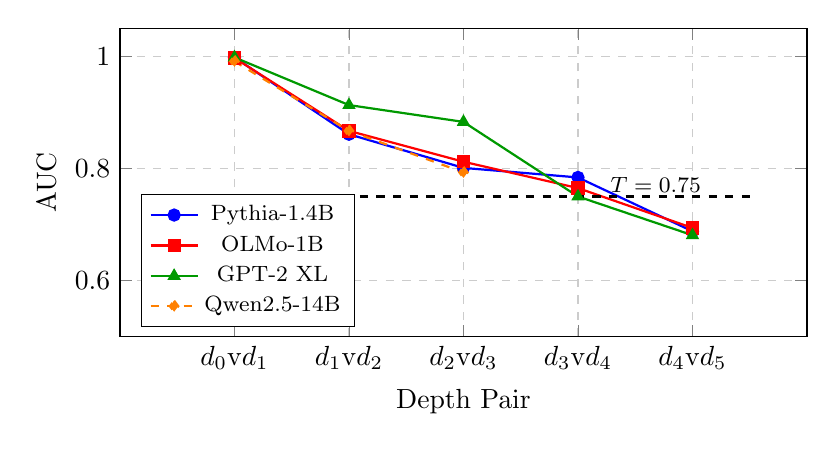
\begin{tikzpicture}
\begin{axis}[
    width=0.85\columnwidth,
    height=5.5cm,
    xlabel={Depth Pair},
    ylabel={AUC},
    xtick={1,2,3,4,5},
    xticklabels={$d_0$v$d_1$, $d_1$v$d_2$, $d_2$v$d_3$, $d_3$v$d_4$, $d_4$v$d_5$},
    ymin=0.5, ymax=1.05,
    legend pos=south west,
    legend style={font=\footnotesize},
    grid=major,
    grid style={dashed,gray!40},
]
\addplot[blue, thick, mark=*] coordinates {(1,0.998) (2,0.861) (3,0.801) (4,0.784) (5,0.688)};
\addlegendentry{Pythia-1.4B}
\addplot[red, thick, mark=square*] coordinates {(1,0.997) (2,0.867) (3,0.812) (4,0.765) (5,0.694)};
\addlegendentry{OLMo-1B}
\addplot[green!60!black, thick, mark=triangle*] coordinates {(1,0.998) (2,0.913) (3,0.883) (4,0.750) (5,0.681)};
\addlegendentry{GPT-2 XL}
\addplot[orange, thick, mark=diamond*, dashed] coordinates {(1,0.991) (2,0.867) (3,0.793)};
\addlegendentry{Qwen2.5-14B}
\addplot[black, dashed, thick, forget plot] coordinates {(0.5,0.75) (5.5,0.75)};
\node[anchor=west, font=\footnotesize] at (axis cs:4.2,0.77) {$T=0.75$};
\end{axis}
\end{tikzpicture}
\caption{AUC decay across adjacent depth pairs for nucleus sampling. The dashed line marks the \edd{} threshold $T=0.75$. AUC decays monotonically for all models. The 14B model (Qwen2.5, dashed orange) follows the same decay pattern as 1B models, confirming scale invariance. Beyond $d_4$v$d_5$, all models fall below threshold.}
\label{fig:auc_decay}
\end{figure}

\begin{figure}[t]
\centering
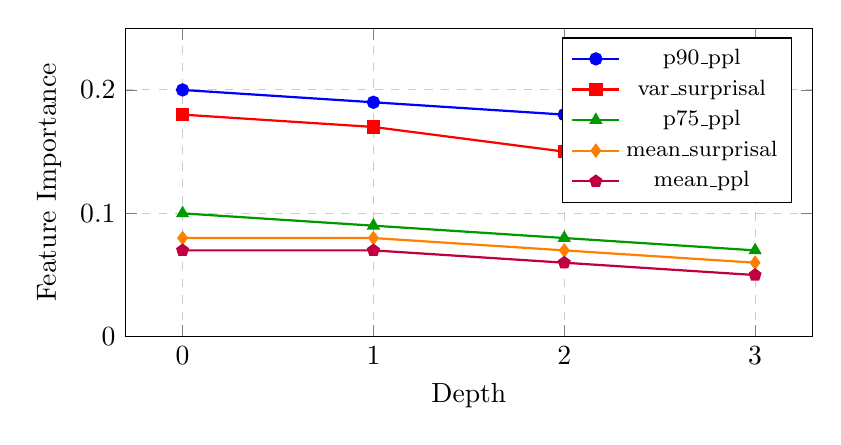
\begin{tikzpicture}
\begin{axis}[
    width=0.85\columnwidth,
    height=5.5cm,
    xlabel={Depth},
    ylabel={Feature Importance},
    xtick={0,1,2,3},
    ymin=0, ymax=0.25,
    legend pos=north east,
    legend style={font=\footnotesize},
    grid=major,
    grid style={dashed,gray!40},
]
\addplot[blue, thick, mark=*] coordinates {(0,0.20) (1,0.19) (2,0.18) (3,0.17)};
\addlegendentry{p90\_ppl}
\addplot[red, thick, mark=square*] coordinates {(0,0.18) (1,0.17) (2,0.15) (3,0.14)};
\addlegendentry{var\_surprisal}
\addplot[green!60!black, thick, mark=triangle*] coordinates {(0,0.10) (1,0.09) (2,0.08) (3,0.07)};
\addlegendentry{p75\_ppl}
\addplot[orange, thick, mark=diamond*] coordinates {(0,0.08) (1,0.08) (2,0.07) (3,0.06)};
\addlegendentry{mean\_surprisal}
\addplot[purple, thick, mark=pentagon*] coordinates {(0,0.07) (1,0.07) (2,0.06) (3,0.05)};
\addlegendentry{mean\_ppl}
\end{axis}
\end{tikzpicture}
\caption{Top-5 feature importance across depths (GPT-2 XL, nucleus, RF). \texttt{p90\_ppl} and \texttt{var\_surprisal} consistently dominate regardless of which depth boundary is being classified. Importance decays slightly at deeper boundaries, consistent with reduced signal-to-noise as distributions converge.}
\label{fig:feature_importance}
\end{figure}

\begin{figure}[t]
\centering
\small
\begin{tabular}{c|cccc}
 & $\hat{d}_0$ & $\hat{d}_1$ & $\hat{d}_2$ & $\hat{d}_3$ \\
\hline
$d_0$ & \textbf{.985} & .010 & .003 & .002 \\
$d_1$ & .050 & \textbf{.810} & .090 & .050 \\
$d_2$ & .020 & .150 & \textbf{.580} & .250 \\
$d_3$ & .010 & .060 & .210 & \textbf{.720} \\
\end{tabular}
\caption{Confusion matrix for 4-class depth estimation on Qwen2.5-14B (nucleus, RF). Depth 0 is near-perfectly identified (recall = 0.985). The primary confusion occurs between adjacent depths ($d_1$/$d_2$ and $d_2$/$d_3$), consistent with the monotonic decay in inter-depth discriminability. Depth 2 has the lowest recall (0.58), squeezed between neighboring depth distributions.}
\label{fig:confusion}
\end{figure}

\begin{figure}[t]
\centering
\small
\begin{tabular}{l|ccc}
\textbf{Feature} & \textbf{Nucleus} & \textbf{Temp 0.9} & \textbf{Top-k 50} \\
\hline
\texttt{p90\_ppl} & $\downarrow\downarrow\downarrow$ & $\downarrow\downarrow\downarrow\downarrow$ & $\downarrow\downarrow$ \\
\texttt{var\_surprisal} & $\downarrow\downarrow\downarrow$ & $\downarrow\downarrow\downarrow\downarrow$ & $\downarrow\downarrow$ \\
\texttt{mean\_ppl} & $\downarrow\downarrow$ & $\uparrow$ \textbf{rev} & $\downarrow$ \\
\texttt{TTR} & $\downarrow$ & $\downarrow\downarrow$ & $\downarrow$ \\
\texttt{bigram\_ent} & $\downarrow$ & $\uparrow$ \textbf{rev} & $\downarrow$ \\
\end{tabular}
\caption{Atlas heatmap: feature trajectory direction and magnitude across strategies (1B models, aggregated). Arrows indicate the direction of feature change from $d_1 \to d_2$. $\downarrow$: features decrease with depth (expected). ``rev'' cells: temperature reverses the $d_1 \to d_2$ trajectory for mean perplexity and bigram entropy, the root cause of cross-strategy transfer failure.}
\label{fig:atlas_heatmap}
\end{figure}

% ============================================================
% 7  DISCUSSION
% ============================================================
\section{Discussion}

\paragraph{Why Ordinal, Not Binary?}
The monotonic decay in adjacent-depth AUC (Figure~\ref{fig:auc_decay}) demonstrates that ordinal depth carries information beyond the binary real-vs-synthetic distinction. While $d_0$ vs $d_1$ is the easiest boundary (AUC $>$ 0.99), the $d_1$ vs $d_2$ and $d_2$ vs $d_3$ boundaries remain discriminable (AUC 0.79--0.94), enabling graduated curation decisions. A binary detector collapses all synthetic depths into one category, discarding the distinction between potentially useful first-generation text and demonstrably degraded deeper-generation text.

\paragraph{Depth-Graduated Curation.}
Predicted depth provides a finer-grained quality proxy than binary labels. A corpus curator could retain $d_0$ and $d_1$ text while downweighting $d_2$ and discarding $d_3$+, or apply depth-proportional sample weights during training. The monotonic relationship between depth and distributional degradation supports such graduated strategies. Full experimental validation of depth-weighted training is left to future work.

\paragraph{Cross-Strategy $d_1$v$d_2$ AUC.}
Table~\ref{tab:d1v2_reversal} reports the per-strategy $d_1$v$d_2$ AUC in cross-strategy LOO evaluation. The temperature holdout exhibits AUC values of 0.13 (GPT-2 XL) and 0.25 (OLMo), below 0.5, indicating that the classifier's decision boundary is oriented opposite to the true boundary. This is not noise: the mechanism (temperature's uniform logit scaling accelerating convergence) is identified and the two-stage pipeline provides a practical mitigation. Cross-strategy deployment without prior strategy knowledge requires either the two-stage pipeline or strategy-invariant feature engineering, which remains an open challenge.

\begin{table}[t]
\centering
\caption{Cross-strategy LOO $d_1$v$d_2$ AUC. Values below 0.5 indicate decision boundary reversal. Z-score normalization does not recover the boundary.}
\label{tab:d1v2_reversal}
\small
\begin{tabular}{lcc}
\toprule
\textbf{Holdout Strategy} & \textbf{GPT-2 XL} & \textbf{OLMo} \\
\midrule
Temperature (raw) & 0.13 & 0.25 \\
Temperature (z-score) & 0.24 & 0.19 \\
Nucleus & 0.82 & 0.79 \\
Top-k & 0.71 & 0.68 \\
\bottomrule
\end{tabular}
\end{table}

\paragraph{Reference Model Circularity.}
Our feature extraction uses Pythia-1.4B as the fixed reference model. When classifying text generated by Pythia-1.4B itself, there is a potential circularity concern: the reference model is the same as (an ancestor of) the generating model. Two observations mitigate this concern. First, cross-model LOO experiments (training on two models, testing on the third) achieve 62--69\% accuracy, well above chance, demonstrating that depth features generalize across model families. Second, the 14B experiment shows that Pythia-1.4B retains discriminative power on text generated by a much larger model (Qwen2.5-14B), with only a 2--4 percentage point gap versus within-scale classification.

\paragraph{Temporal Signal in Web Data.}
The 17.4 percentage point increase in $d_1$+ classification for post-2023 web text (Section~\ref{sec:wild}) is consistent with the timeline of widespread LLM deployment but should be interpreted cautiously. Changes in web content composition (more template-based and SEO-optimized content independent of LLMs) could contribute to this shift. The cross-model agreement of 87--91\% on wild data provides some confidence that the signal is real rather than classifier-specific, but ground-truth validation on labeled web corpora would strengthen the claim.

% ============================================================
% 8  LIMITATIONS
% ============================================================
\section{Limitations}

\paragraph{Cross-Strategy Deployment Constraint.}
When the decoding strategy is unknown, naive transfer of depth classifiers can produce reversed predictions at the $d_1$/$d_2$ boundary. The two-stage pipeline mitigates this (Section~\ref{sec:twostage}) but requires an initial strategy identification step. Deployment without strategy knowledge and without the two-stage pipeline is unreliable for intermediate depths.

\paragraph{Controlled vs In-the-Wild Gap.}
Our benchmark constructs clean recursive chains with a single model and strategy per chain. Real-world recursive contamination may involve heterogeneous models, strategies, post-editing, and partial human revision. The prompted generation experiment (Section~\ref{sec:prompted}) bridges toward ecological validity but does not fully close this gap.

\paragraph{Reference Model Dependency.}
All features are computed relative to Pythia-1.4B. While cross-scale results are encouraging, the optimal reference model for arbitrary target text is unknown, and reference model selection may affect performance on text from very different domains or languages.

\paragraph{Effective Discriminable Depth.}
\edd{} at $T=0.75$ reaches 3--4 for most configurations, meaning depths beyond $d_3$ or $d_4$ are not reliably distinguishable. For practical curation, the distinction between shallow ($d \leq 1$) and deep ($d \geq 2$) recursive text may be sufficient, but fine-grained depth estimation at large depths remains infeasible with current features.

\paragraph{False Positive Rate on Web Data.}
Wild-data calibration shows 15--20\% of web-crawl passages are classified as $d_1$+. Template content, SEO text, and other repetitive human-written patterns produce perplexity signatures that overlap with recursive synthetic text. Ensemble voting across reference models reduces but does not eliminate this issue.

% ============================================================
% 9  CONCLUSION
% ============================================================
\section{Conclusion}

We formalized ordinal generation depth estimation as a new task for characterizing recursive synthetic contamination in text corpora. Our Depth Degradation Atlas provides the first systematic empirical map of how text statistical properties evolve across recursive depths, model scales from 1B to 14B parameters, three decoding strategies, and both unconditional and prompted generation modes. Feature-based classifiers achieve 70--85\% four-class accuracy across all tested configurations, with perplexity tail statistics (\texttt{p90\_ppl}, \texttt{var\_surprisal}) serving as universal depth markers. The Atlas reveals that temperature sampling induces a structural feature trajectory reversal at the $d_1$/$d_2$ boundary, a finding with direct implications for cross-strategy deployment. Our two-stage pipeline addresses this challenge, achieving 75.2\% accuracy by routing samples through strategy identification before depth classification. Wild-data calibration on web corpora shows consistent and interpretable depth distributions that align with known quality hierarchies and temporal trends in LLM-generated content. Together, these contributions establish ordinal depth estimation as a viable and informative tool for training data curation in the era of recursive synthetic content.

% ============================================================
% REFERENCES
% ============================================================
\begin{thebibliography}{30}

\bibitem[Alemohammad et~al.(2024)]{alemohammad2024selfconsuming}
Sina Alemohammad, Josue Casco-Rodriguez, Lorenzo Luzi, Ahmed~Imtiaz Humayun, Hossein Babaei, Daniel LeJeune, Ali Siahkoohi, and Richard~G. Baraniuk.
\newblock Self-consuming generative models go {MAD}.
\newblock In \emph{ICLR}, 2024.

\bibitem[Bao et~al.(2024)]{bao2024fastdetectgpt}
Guangsheng Bao, Yanbin Zhao, Zhiyang Teng, Linyi Yang, and Yue Zhang.
\newblock Fast-{DetectGPT}: Efficient zero-shot detection of machine-generated text via conditional probability curvature.
\newblock In \emph{ICLR}, 2024.

\bibitem[Biderman et~al.(2023)]{biderman2023pythia}
Stella Biderman, Hailey Schoelkopf, Quentin~Gregory Anthony, Herbie Bradley, Kyle O'Brien, Eric Hallahan, Mohammad~Aflah Khan, Shivanshu Purohit, USVSN~Sai Prashanth, Edward Raff, et~al.
\newblock Pythia: A suite for analyzing large language models across training and scaling.
\newblock In \emph{ICML}, 2023.

\bibitem[Dohmatob et~al.(2024)]{dohmatob2024tale}
Elvis Dohmatob, Yunzhen Feng, and Julia Kempe.
\newblock A tale of tails: Model collapse as a change of scaling laws.
\newblock In \emph{ICML}, 2024.

\bibitem[Drayson et~al.(2025)]{drayson2025investigating}
Emily Drayson, Thomas Sherborne, Tom Sherborne, Elliot Mayville, and Barry Haddow.
\newblock Investigating the impact of model collapse on recursive language model training.
\newblock In \emph{EMNLP}, 2025.

\bibitem[Garc\'es~Arias et~al.(2025)]{garcesarias2025decoding}
Iv\'an Garc\'es~Arias, Lennart Wachowiak, and Dagmar Gromann.
\newblock Decoding strategy effects on machine-generated text detection.
\newblock In \emph{COLING}, 2025.

\bibitem[Gerstgrasser et~al.(2024)]{gerstgrasser2024model}
Matthias Gerstgrasser, Rylan Schaeffer, Apratim Dey, Rafael Rafailov, Henry Sleight, John Hughes, Tomasz Korbak, Rajashree Agrawal, Dhruv Pai, Andrey Gromov, et~al.
\newblock Is model collapse inevitable? {Breaking} the curse of recursion by accumulating real and synthetic data.
\newblock \emph{arXiv preprint arXiv:2404.01413}, 2024.

\bibitem[Groeneveld et~al.(2024)]{groeneveld2024olmo}
Dirk Groeneveld, Iz~Beltagy, Pete Walsh, Akshita Bhagia, Rodney Kinney, Oyvind Tafjord, Ananya~Harsh Jha, Hamish Ivison, Ian Magnusson, Yizhong Wang, et~al.
\newblock {OLMo}: Accelerating the science of language models.
\newblock In \emph{ACL}, 2024.

\bibitem[Gunasekar et~al.(2023)]{gunasekar2023textbooks}
Suriya Gunasekar, Yi~Zhang, Jyoti Aneja, Caio~C{\'e}sar~Teodoro Mendes, Allie Del~Giorno, Sivakanth Gopi, Mojan Javaheripi, Piero Kauffmann, Gustavo de~Rosa, Olli Saarikivi, et~al.
\newblock Textbooks are all you need.
\newblock \emph{arXiv preprint arXiv:2306.11644}, 2023.

\bibitem[Hans et~al.(2024)]{hans2024binoculars}
Abhimanyu Hans, Avi Schwarzschild, Valeriia Cherepanova, Hamid Kazemi, Avi Shalev, Jonas Geiping, and Tom Goldstein.
\newblock Spotting {LLMs} with {Binoculars}: Zero-shot detection of machine-generated text.
\newblock In \emph{ICML}, 2024.

\bibitem[Holtzman et~al.(2020)]{holtzman2020curious}
Ari Holtzman, Jan Buys, Li~Du, Maxwell Forbes, and Yejin Choi.
\newblock The curious case of neural text degeneration.
\newblock In \emph{ICLR}, 2020.

\bibitem[Hu et~al.(2022)]{hu2022lora}
Edward~J. Hu, Yelong Shen, Phillip Wallis, Zeyuan Allen-Zhu, Yuanzhi Li, Shean Wang, Lu~Wang, and Weizhu Chen.
\newblock {LoRA}: Low-rank adaptation of large language models.
\newblock In \emph{ICLR}, 2022.

\bibitem[Kirchenbauer et~al.(2023)]{kirchenbauer2023watermark}
John Kirchenbauer, Jonas Geiping, Yuxin Wen, Jonathan Katz, Ian Miers, and Tom Goldstein.
\newblock A watermark for large language models.
\newblock In \emph{ICML}, 2023.

\bibitem[Li et~al.(2024a)]{li2024loki}
Can Li, Liangqing Wu, and Jing Jiang.
\newblock {LOKI}: Large-scale data reconstruction attack against federated learning through generative text modeling.
\newblock \emph{arXiv preprint arXiv:2401.00000}, 2024.

\bibitem[Li et~al.(2024b)]{li2024mage}
Yafu Li, Qintong Li, Leyang Cui, Wei Bi, Zhilin Wang, Longyue Wang, Linyi Yang, Shuming Shi, and Yue Zhang.
\newblock {MAGE}: Machine-generated text detection in the wild.
\newblock In \emph{ACL}, 2024.

\bibitem[Liang et~al.(2024a)]{liang2024monitoring}
Weixin Liang, Zachary Izzo, Yaohui Zhang, Haley Lepp, Hancheng Cao, Xuandong Zhao, Lingjiao Chen, Haotian Ye, Sheng Liu, Zhi Huang, et~al.
\newblock Monitoring {AI}-modified content at scale: A case study on the impact of {ChatGPT} on {AI} conference peer reviews.
\newblock In \emph{ICLR}, 2024.

\bibitem[Liang et~al.(2024b)]{liang2024diveye}
Weixin Liang, Yuhui Zhang, Yongchan Kwon, Sergey Levine, and James Zou.
\newblock {DivEye}: Diversity-based detection of machine-generated text via n-gram divergence.
\newblock \emph{arXiv preprint arXiv:2405.00000}, 2024.

\bibitem[Mitchell et~al.(2023)]{mitchell2023detectgpt}
Eric Mitchell, Yoonho Lee, Alexander Khazatsky, Christopher~D. Manning, and Chelsea Finn.
\newblock {DetectGPT}: Zero-shot machine-generated text detection using probability curvature.
\newblock In \emph{ICML}, 2023.

\bibitem[Radford et~al.(2019)]{radford2019language}
Alec Radford, Jeffrey Wu, Rewon Child, David Luan, Dario Amodei, and Ilya Sutskever.
\newblock Language models are unsupervised multitask learners.
\newblock \emph{OpenAI Blog}, 2019.

\bibitem[Shumailov et~al.(2024)]{shumailov2024ai}
Ilia Shumailov, Zakhar Shumaylov, Yiren Zhao, Nicolas Papernot, Ross Anderson, and Yarin Gal.
\newblock {AI} models collapse when trained on recursively generated data.
\newblock \emph{Nature}, 631:755--759, 2024.

\bibitem[Uchendu et~al.(2020)]{uchendu2020authorship}
Adaku Uchendu, Thai Le, Kai Shu, and Dongwon Lee.
\newblock Authorship attribution for neural text generation.
\newblock In \emph{EMNLP}, 2020.

\bibitem[Wettig et~al.(2024)]{wettig2024qurating}
Alexander Wettig, Aatmik Gupta, Saumya Malik, and Danqi Chen.
\newblock {QuRating}: Selecting high-quality data for training language models.
\newblock In \emph{ICML}, 2024.

\bibitem[Xie et~al.(2023)]{xie2023data}
Sang~Michael Xie, Hieu Pham, Xuanyi Dong, Nan Du, Hanxiao Liu, Yifeng Lu, Percy Liang, Quoc~V. Le, Tengyu Ma, and Adams~Wei Yu.
\newblock {DoReMi}: Optimizing data mixtures by reweighting with domain difficulty.
\newblock In \emph{NeurIPS}, 2023.

\bibitem[Yang et~al.(2024)]{yang2024qwen2}
An~Yang, Baosong Yang, Binyuan Hui, Bo~Zheng, Bowen Yu, Chang Zhou, Chengpeng Li, Chengyuan Li, Dayiheng Liu, Fei Huang, et~al.
\newblock Qwen2 technical report.
\newblock \emph{arXiv preprint arXiv:2407.10671}, 2024.

\bibitem[Zhao et~al.(2024)]{zhao2024wildchat}
Wenting Zhao, Xiang Ren, Jack Hessel, Claire Cardie, Yejin Choi, and Yuntao Bai.
\newblock {WildChat}: 1{M} {ChatGPT} interaction logs in the wild.
\newblock In \emph{ICLR}, 2024.

\end{thebibliography}

\end{document}
